%% Verze pro jednostranný tisk:
% Okraje: levý 40mm, pravý 25mm, horní a dolní 25mm
% (ale pozor, LaTeX si sám přidává 1in)
\documentclass[12pt,a4paper]{article}

% \openright zařídí, aby následující text začínal na pravé straně knihy
%\let\openright=\clearpage

%% Pokud tiskneme oboustranně:
% \documentclass[12pt,a4paper,twoside,openright]{report}
% \setlength\textwidth{145mm}
% \setlength\textheight{247mm}
% \setlength\oddsidemargin{14.2mm}
% \setlength\evensidemargin{0mm}
% \setlength\topmargin{0mm}
% \setlength\headsep{0mm}
% \setlength\headheight{0mm}
% \let\openright=\cleardoublepage

%% Vytváříme PDF/A-2u
\usepackage[a-2u]{pdfx}

%% Přepneme na českou sazbu a fonty Latin Modern
\usepackage[slovak]{babel}
\usepackage{lmodern}
\usepackage[IL2]{fontenc}%T1
\usepackage{textcomp}
\usepackage{hyperref}

\usepackage{float}
\usepackage{subfigure}

%% Použité kódování znaků: obvykle latin2, cp1250 nebo utf8:
\usepackage[utf8]{inputenc}

%%% Další užitečné balíčky (jsou součástí běžných distribucí LaTeXu)
\usepackage{amsmath}        % rozšíření pro sazbu matematiky
\usepackage{amsfonts}       % matematické fonty
\usepackage{amsthm}         % sazba vět, definic apod.

%bolo treba vypnut kvoli rozdelovaniu
%\usepackage{bbding}         % balíček s nejrůznějšími symboly
% (čtverečky, hvězdičky, tužtičky, nůžtičky, ...)
\usepackage{bm}             % tučné symboly (příkaz \bm)
\usepackage{graphicx}       % vkládání obrázků
\usepackage{fancyvrb}       % vylepšené prostředí pro strojové písmo
\usepackage{indentfirst}    % zavede odsazení 1. odstavce kapitoly
%\usepackage{natbib}         % zajištuje možnost odkazovat na literaturu
% stylem AUTOR (ROK), resp. AUTOR [ČÍSLO]
\usepackage[nottoc]{tocbibind} % zajistí přidání seznamu literatury,
% obrázků a tabulek do obsahu
\usepackage{icomma}         % inteligetní čárka v maltematickém módu
\usepackage{dcolumn}        % lepší zarovnání sloupců v tabulkách
\usepackage{booktabs}       % lepší vodorovné linky v tabulkách
\usepackage{paralist}       % lepší enumerate a itemize
\usepackage[usenames]{xcolor}  % barevná sazba

\usepackage{url}

\usepackage{pdfpages}
%opening
\title{}
\author{}

\begin{document}
	\pagestyle{empty}
\section{Fibbonacciho halda}

\subsection{Porovnanie počtu krokov operácie delete min rovnomerného a nevyváženého testu pri štandardnej implementácii}

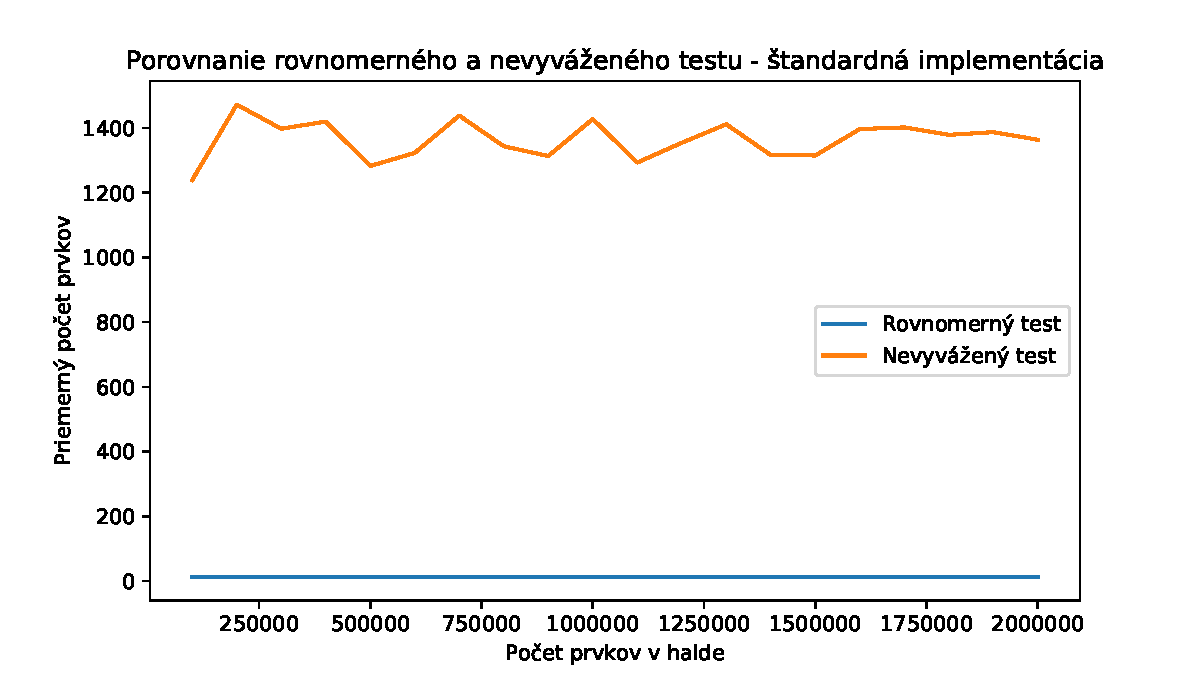
\includegraphics[width=\linewidth]{1.pdf}

Obe krivky vyzerajú na grafe konštantne vzhľadom na počet prvkov v halde. Pri nevyváženom teste majú hodnoty príliš veľký rozptyl aby sa o nich niečo dalo definitívne povedať, čo je spôsobené tým, že pri generovaní používame náhodu. Pri bližšom skúmaní hodnôt priemerného počtu krokov v rovnomernom teste môžeme povedať, že počet krokov rastie, hoci pomaly.

Z teórie vieme, že amortizovaná časová zložitosť operácie delete min je $\mathcal{O}(\log{}n)$, čo na grafe nevieme pozorovať. Dôvodom je pravdepodobne veľká konštanta skrytá v asymptotickej zložitosti.

V nevyváženom teste je taký veľký priemer, pretože sa volá operácie delete min menej často a teda vždy potrebuje veľa krokov na konsolidáciu haldy (medzitým sa vykonali iné operácie).

\subsection{Porovnanie implementácii v zákernom teste}

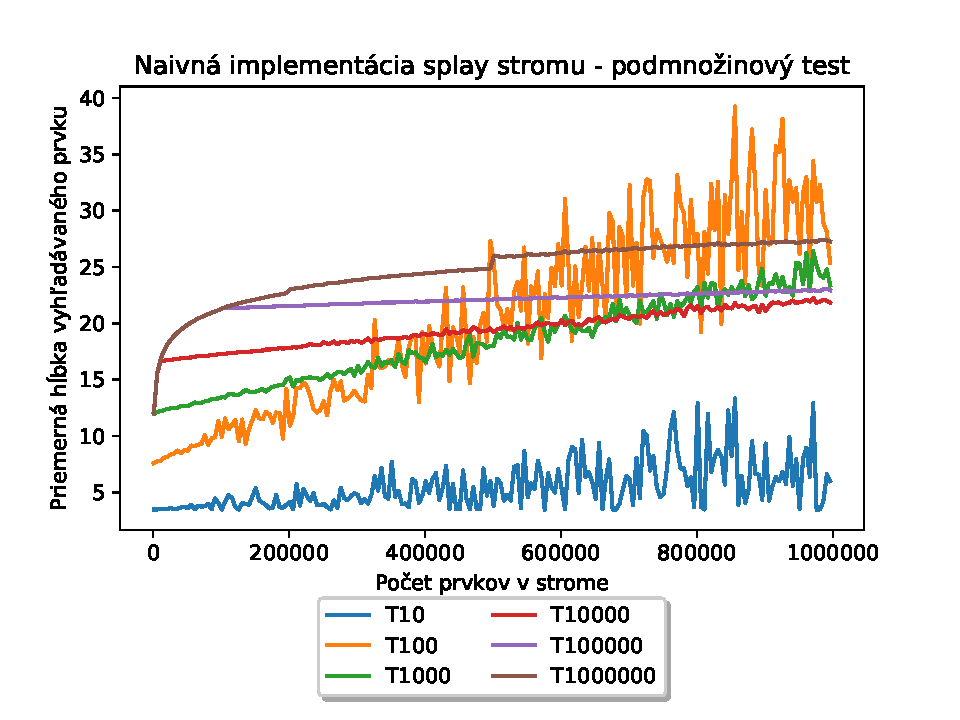
\includegraphics[width=\linewidth]{2.pdf}

Tento test demonštruje to, že zložitosť operácie delete min v najhoršom prípade pri naivnej halde je $\mathcal{O}(\sqrt{n})$, a nepomôže nám ani amortizácia.

Pri naivnej verzii dokážeme istou postupnosťou operácii dosiahnuť, že halda bude obsahovať (rádovo) $\sqrt{n}$ stromov hĺbky 2, každý iného rádu. Prvý strom pozostáva iba z jedného vrchola, druhý je vrchol s jedným synom, tretí je s 2 synmi, atd. Posledný má rádovo $\sqrt{n}$ synov. V takejto halde dokážeme opakovať ľubovoľne veľa operácii \texttt{Insert x} a \texttt{DeleteMin}, kde x je nejaký kľúč menší ako všetky ostatné v halde. Delete min musí nájsť nové minimum a preto musí prejsť až $\sqrt{n}$ synov.

V implementácii však nepočítame kroky pri hľadaní minima. Generátor najskôr uvedie haldu do stavu opísaného vyššie a potom posiela halde veľa krát za sebou túto postupnosť krokov:
\begin{enumerate}
	\item \texttt{Insert x}
	\item \texttt{Insert x-1}
	\item \texttt{DeleteMin}
	\item \texttt{DeleteMin}
\end{enumerate}
kde x a x-1 sú dva najmenšie prvky v halde. Prvé \texttt{DeleteMin} spôsobí konsolidáciu v halde, výsledkom ktorej je jeden strom, ktorý má ako deti korene stromov pred konsolidáciou. Druhé \texttt{DeleteMin} odstráni koreň jediného stromu, a vráti haldu do pôvodného stavu. Prvé \texttt{DeleteMin} spravilo (rádovo) $\sqrt{n}$ krokov.

V štandardnej implementácii tento postup nevytvorí príliš veľa plytkých stromov, a teda pozorujeme konštantný počet krokov. Pri opakovaní vyššie vymenovaných krokov nastane konsolidácia pri prvom \texttt{DeleteMin}, ktorá trvá, kým sa nenájde pre novo zlúčený strom miesto. Mohla by trvať až log n krokov, no zjavne sa vždy nájde miesto medzi stromami malého rádu.


\subsection{Porovnanie maximálneho a priemerného počtu krokov operácii naivnej a štandardnej implementácie v hlbokom teste}

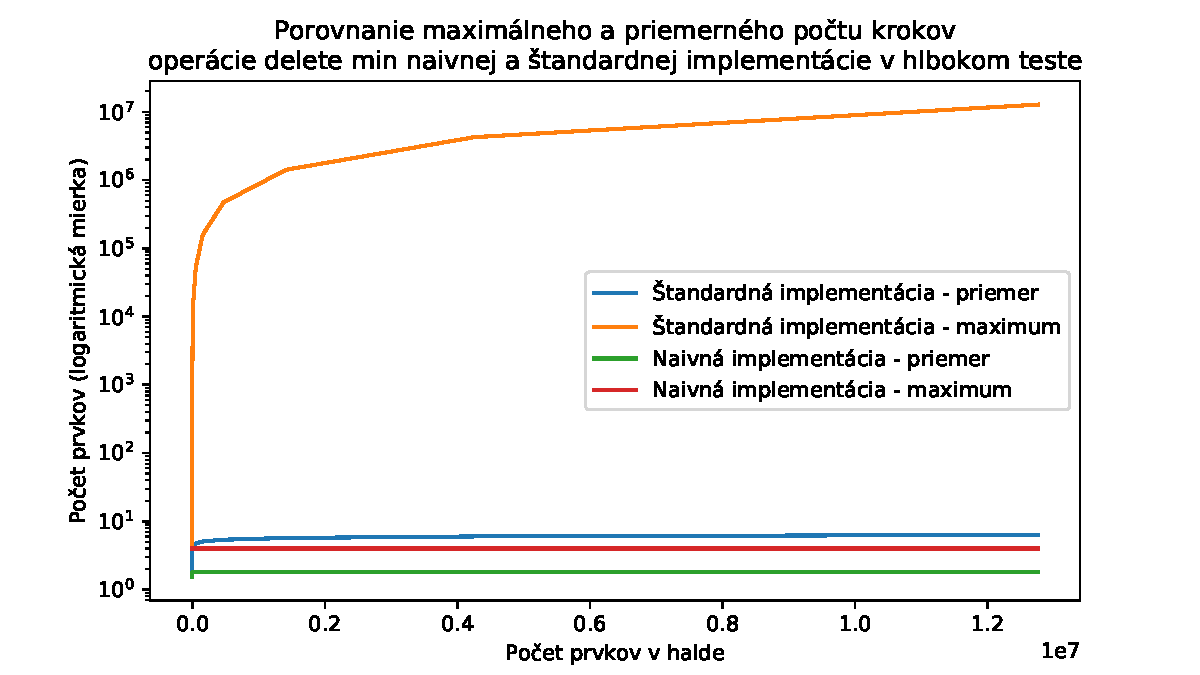
\includegraphics[width=\linewidth]{3.pdf}

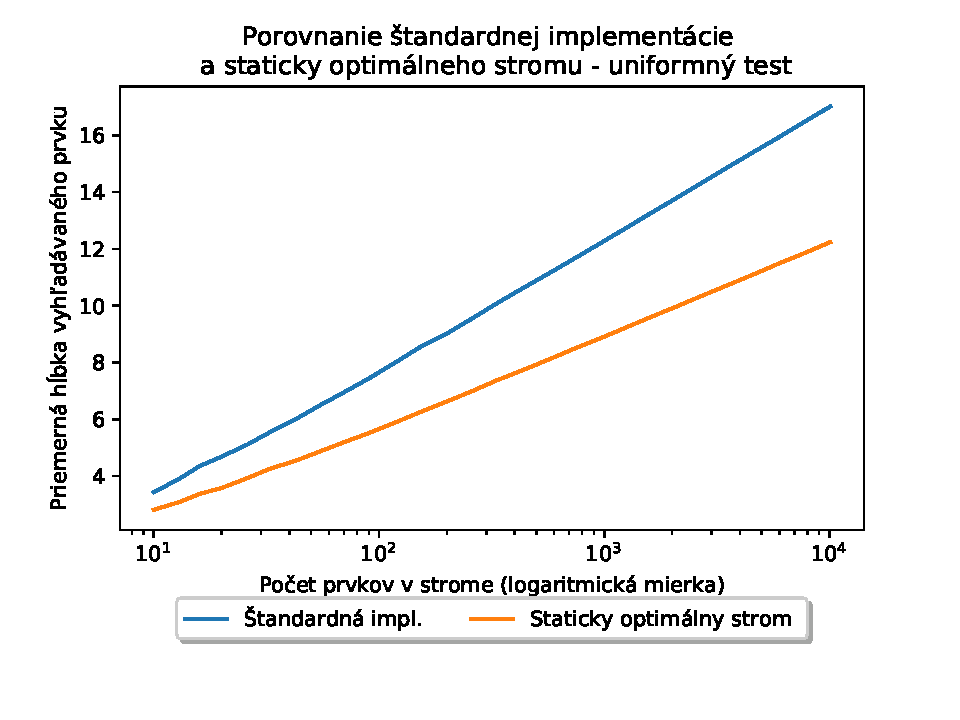
\includegraphics[width=\linewidth]{4.pdf}

Z grafov vidíme, že maximum krokov oboch operácii štandardnej implementácie rastie lineárne (logaritmickú mierku som použil, by bolo vidieť rozdiel medzi zvyšnými krivkami). Ostatné závislosti sú konštantné.

Operácie v hlbokom teste postavia z vrcholov haldy cestu, v ktorej je každý vrchol označený. Na konci zavolá operácie \texttt{Decrease} na najhlbší prvok cesty a \texttt{DeleteMin}. Počas stavania cesty potrebuje každá operácia konštantný počet krokov.

V štandardnej implementácii \texttt{Decrease} spôsobí, že celá cesta sa rozpadne na stromy rádu 0, na čo potrebujeme (približne) n krokov. Následný \texttt{DeleteMin} spôsobí konsolidáciu, ktorá trvá (približne) n krokov. To teda potvrdzuje worst case zložitosť operácii: $\mathcal{O}(n)$. V priemere však má \texttt{Decrease} zaručenú zložitosť $\mathcal{O}(1)$, čo potvrdzuje graf. \texttt{DeleteMin} má v tomto špeciálnom teste konštantnú amortizovanú zložitosť. 

V naivnej implementácii \texttt{Decrease} jednoducho odtrhne posledný vrchol cesty a \texttt{DeleteMin} odstráni buď tento vrchol alebo koreň cesty, na čo potrebujeme konštantný počet krokov. Decrease naivnej implementácie potrebuje vždy práve jeden krok. 



\end{document}